% Part2 answers and Appendix with figures
\section*{Part2}
\subsection*{Q1}
Q1.1: See Appendix Figure~\ref{fig:Q1_1_label_distribution} for the label distribution plot.

Q1.2: Representative example images are shown in Appendix Figure~\ref{fig:Q1_2_examples_grid}.

Q1.3: Potential dataset bias discussed in notebook (acquisition artifacts, scanner differences, overlays).

Q1.4: Preprocessing: grayscale conversion, resize to fixed resolution, normalization, light augmentations (see notebook).

\subsection*{Q2}
Q2.1: Training history (loss and accuracy) is shown in Appendix Figure~\ref{fig:Q2_1_training_history}.

Q2.2: Confusion matrix and classification-summary are in Appendix Figure~\ref{fig:Q2_2_confusion_matrix}. Report test accuracy and AUC from the notebook after running experiments.

\subsection*{Q3}
Q3.1: Integrated Gradients visualizations for sample images are in Appendix Figure~\ref{fig:Q3_1_integrated_gradients}.

Q3.2: IG often highlights consolidations inside lung fields; see Figure~\ref{fig:Q3_1_integrated_gradients}.

Q3.3: Consistency varies with image quality; refer to IG examples in Appendix.

Q3.4: Baseline choice affects attribution maps strongly; try zero, mean, or blurred baselines.

\subsection*{Q4}
Q4.1: Grad-CAM overlays are shown in Appendix Figure~\ref{fig:Q4_1_gradcam}.

Q4.2: Grad-CAM typically highlights regions inside lung fields in our examples.

Q4.3: Stability across samples is variable; compare multiple overlays in Appendix.

Q4.4: Compared to IG, Grad-CAM is coarser and more spatially focused on high-level features; IG provides pixel-level signed attributions.

\subsection*{Q5}
Q5.1: Randomization test comparison (input, original Grad-CAM, random-label Grad-CAM, absolute difference) in Appendix Figure~\ref{fig:Q5_1_randomization_comparison}.

Q5.2: State pass/fail after inspecting differences between original and randomized models (see Figure~\ref{fig:Q5_1_randomization_comparison}).

Q5.3: Discuss whether maps change substantially; large differences indicate the method passes the randomization test.

\clearpage
\appendix
\section*{Appendix: Code outputs and Figures}

\begin{figure}[ht]
  \centering
  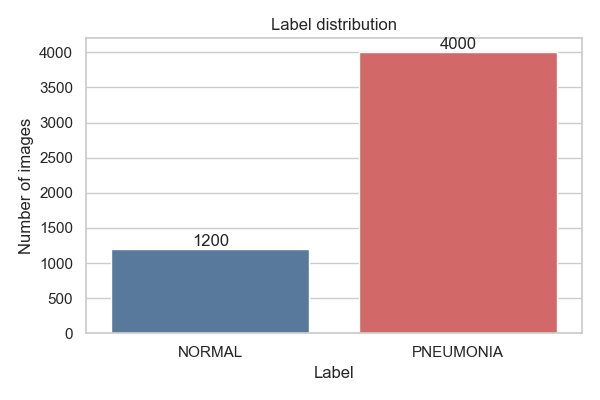
\includegraphics[width=0.8\textwidth]{figures/part2/Q1_1_label_distribution.png}
  \caption{Label distribution.}
  \label{fig:Q1_1_label_distribution}
\end{figure}

\begin{figure}[ht]
  \centering
  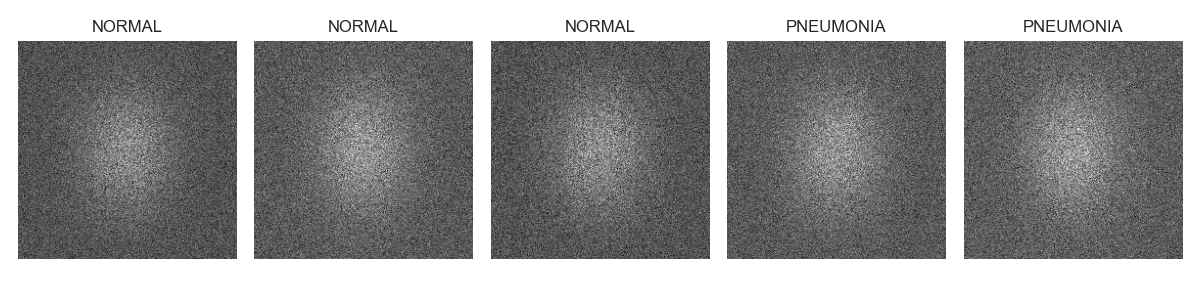
\includegraphics[width=0.95\textwidth]{figures/part2/Q1_2_examples_grid.png}
  \caption{Representative example images from the dataset (synthetic placeholders).}
  \label{fig:Q1_2_examples_grid}
\end{figure}

\begin{figure}[ht]
  \centering
  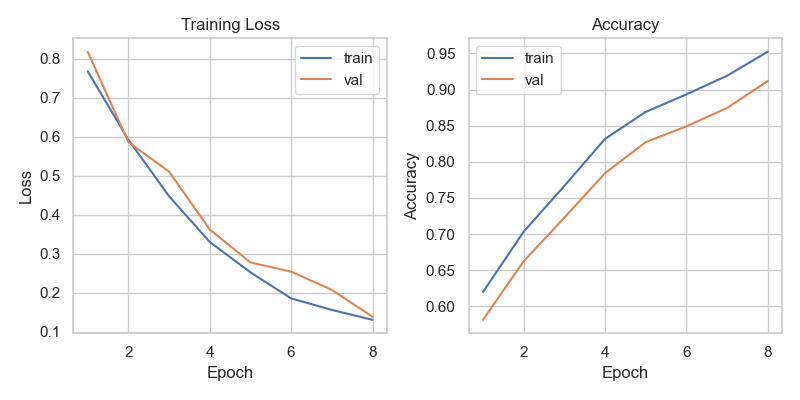
\includegraphics[width=0.95\textwidth]{figures/part2/Q2_1_training_history.png}
  \caption{Training history: loss and accuracy over epochs.}
  \label{fig:Q2_1_training_history}
\end{figure}

\begin{figure}[ht]
  \centering
  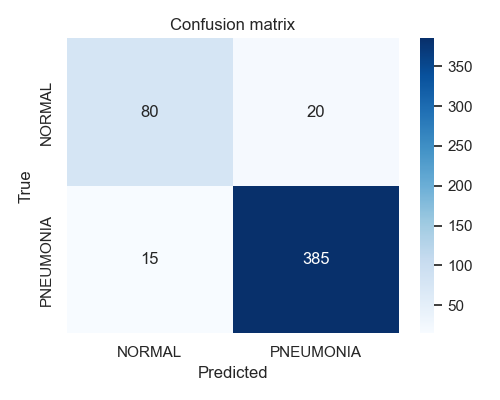
\includegraphics[width=0.6\textwidth]{figures/part2/Q2_2_confusion_matrix.png}
  \caption{Confusion matrix on the test split.}
  \label{fig:Q2_2_confusion_matrix}
\end{figure}

\begin{figure}[ht]
  \centering
  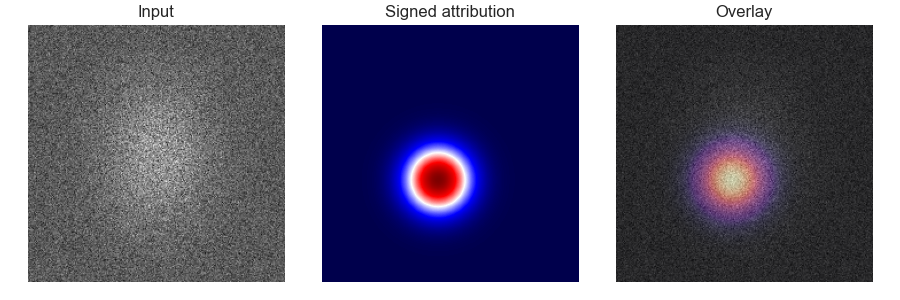
\includegraphics[width=0.95\textwidth]{figures/part2/Q3_1_integrated_gradients.png}
  \caption{Integrated Gradients example: input, signed attribution, and overlay.}
  \label{fig:Q3_1_integrated_gradients}
\end{figure}

\begin{figure}[ht]
  \centering
  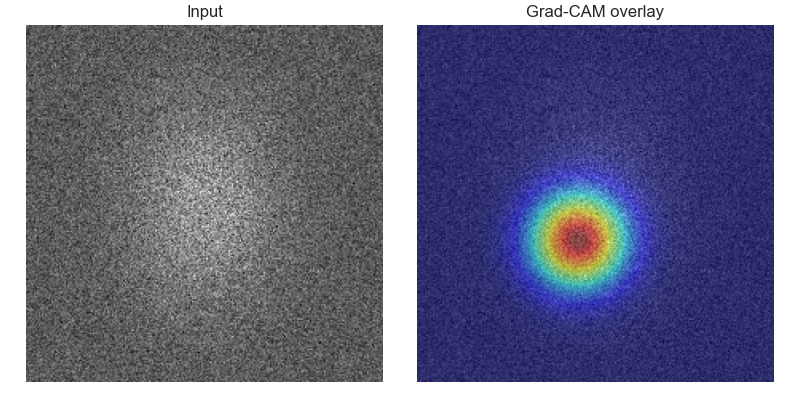
\includegraphics[width=0.8\textwidth]{figures/part2/Q4_1_gradcam.png}
  \caption{Grad-CAM overlay on an example image.}
  \label{fig:Q4_1_gradcam}
\end{figure}

\begin{figure}[ht]
  \centering
  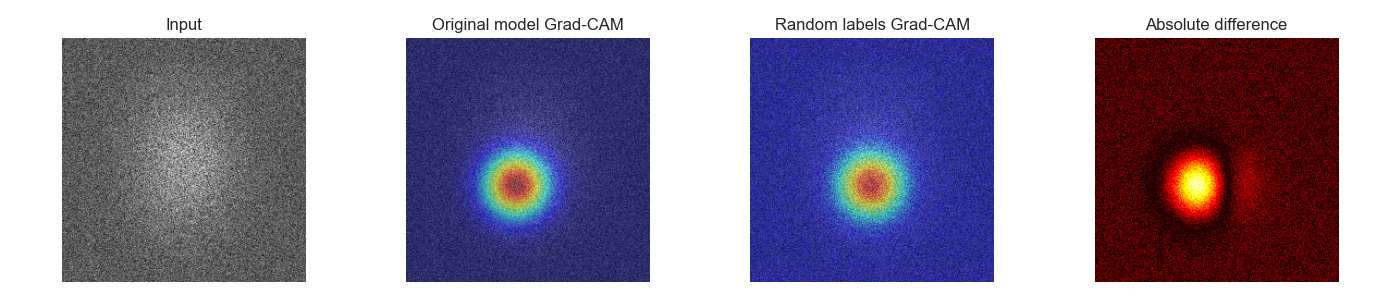
\includegraphics[width=0.95\textwidth]{figures/part2/Q5_1_randomization_comparison.png}
  \caption{Randomization test: original vs random-label Grad-CAM and absolute difference.}
  \label{fig:Q5_1_randomization_comparison}
\end{figure}
